\chapter{System design}
\section{Overview}

In this chapter we will describe the design of the system from components and architectural point. The system design and architecture will rely on the requirements, actors and the enviroment overall. This description will give enough information about the system and it's components and overview how the real world implementation will look like.

\section{System design}
	\subsection{System decomposition}

Kitab is composed of 4 componenets as shown in the graphic below. In this way the system will be more realizable as different components. Figure~\ref{dia_sys_decomposition} shows how we decomposed kitab.

	\begin{figure}[H]
	\begin{center}

	\tcbox{\includegraphics[width=10cm]{"Diagram/System Decomposition".png}}
	\caption{System decomposition diagram for kitab}
	\label{dia_sys_decomposition}

	\end{center}
	\end{figure}

	\subsection{Module Description}

	\begin{enumerate}
		\item Content management
		\item User management
		\item Kitab service
		\item Kitab app
	\end{enumerate}

\section{Architecture}
	\subsection{Architectural Style and Pattern}

		\subsubsection{Architectural style}

		\begin{description}
			\item[Pipe-Filter architectural style] - is an architectural style in which different processing components form a chain so that the output of one component can be input to the following one.
			
			\item[Client-Server architectural style] - is an architectural style in which division of components where the client intiates a communication and requests different resources and the server responds to the request.
			
			\item[Publish-Subscribe architectural style] - is an architectural style in which senders of messages(publishers) publish messages with out knowing the recipient component.
		\end{description}

		\subsubsection{Architectural pattern}

		\begin{description}
			\item[Model-View-Controller architectural pattern] - This architectural pattern the main components in the system implementation are divided as :-
			\begin{description}
				\item[Model] - component that holds persistent data. \\
				In our case - database to store all the applications' data and it's abstraction as an ORM.
				\item[View] - component that works what the user will see and how the data could be presentable.\\
				In our case - interfaces for the web and mobile client application.
				\item[Controller] - component that controls the system state and interaction with the outside enviroment.\\
				In our case - the gin web server and buffalo router as a backend.
			\end{description}
			The figure~\ref{dia_mvc_arch_pattern} shows how "MVC" architectural pattern is used in the system.
		\end{description}

		\begin{figure}[H]
		\begin{center}

		\tcbox{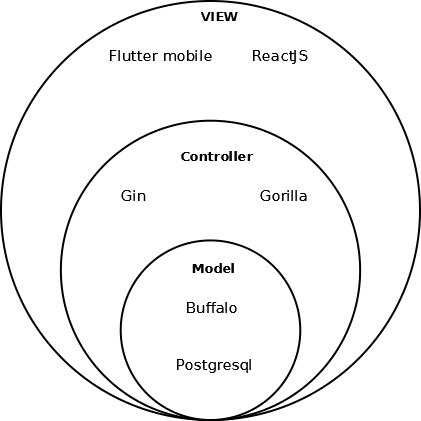
\includegraphics[width=7cm]{Diagram/MVC.png}}
		\caption{MVC architectural pattern for kitab}
		\label{dia_mvc_arch_pattern}

		\end{center}
		\end{figure}

	\subsection{Component Diagram}

	\subsection{Deployment Diagram}

\section{Database design}

\section{User-interface design}